\section{Experimental Results and Analysis}
\label{sec:results}

Our experiments were designed to evaluate both the performance and the predictive accuracy of our 
optimized GRU-ODE-Bayes model against a strong baseline.

\subsection{The GPU Performance Anomaly}

Despite our vectorization efforts, we observed a baffling performance characteristic: 
the model trained significantly slower on a high-end GPU than on a CPU.
\begin{itemize}
    \item \textbf{CPU Training Time (batch size 1):} $\sim$1 hour / epoch.
    \item \textbf{GPU Training Time (batch size 64):} $\sim$5 hours / epoch.
\end{itemize}

Systematic profiling revealed that the bottleneck was the \texttt{odeint\_adjoint} function itself. 
For this model's specific workload—solving many short ODE segments back-to-back—the fixed overhead of 
launching CUDA kernels and managing the adjoint state on the GPU dominated the actual computation. 
The CPU, with its lower call overhead for sequential tasks, proved more efficient for this particular operational pattern.

\subsection{Model Accuracy and Baseline Comparison}

The most critical part of our analysis was comparing the full GRU-ODE-Bayes model against 
a simple but powerful baseline. 
This baseline uses the exact same architecture but \textbf{removes the ODE solver}, 
replacing it with a simple identity function that carries the last hidden state forward. 
The results were stark, as shown in Table~\ref{tab:results}.

\begin{table}[h]
  \centering
  \caption{Performance and Accuracy Comparison.}
  \label{tab:results}
  \begin{tabular}{l c c}
    \toprule
    \textbf{Metric} & \textbf{GRU-ODE-Bayes} & \textbf{Baseline (No ODE)} \\
    \midrule
    Validation Accuracy & 62.0\% & \textbf{97.78\%} \\
    Training Time / Epoch & $\sim$1 hour (CPU) & $\sim$30 seconds \\
    \bottomrule
  \end{tabular}
\end{table}

The complex, theoretically-motivated GRU-ODE-Bayes model was not only 120 times slower but also drastically 
less accurate than the simple baseline. 
The continuous dynamics modeled by the ODE solver did not provide a useful inductive bias for this classification task; 
instead, it appears to have hindered learning, possibly by introducing numerical instability or an overly complex loss landscape.

\subsection{A Successful Application: Learning Dynamical Systems}

To isolate and demonstrate the power of the NODE concept for its intended purpose, we conducted a 
supplementary experiment on a classic dynamical systems problem: 
learning the dynamics of the Lotka-Volterra (prey-predator) model. 
Here, the task is not classification, but to learn the underlying vector field from sparse trajectory data.

We first compare the ground truth dynamics to the output of a standard Multi-Layer Perceptron (MLP) with a similar number of parameters. 
As shown in Figure~\ref{fig:lv_true_vs_mlp}, the standard MLP is unable to learn the rotational structure of the system,
demonstrating its lack of an appropriate inductive bias for this task.

\begin{figure}[h!]
  \centering
  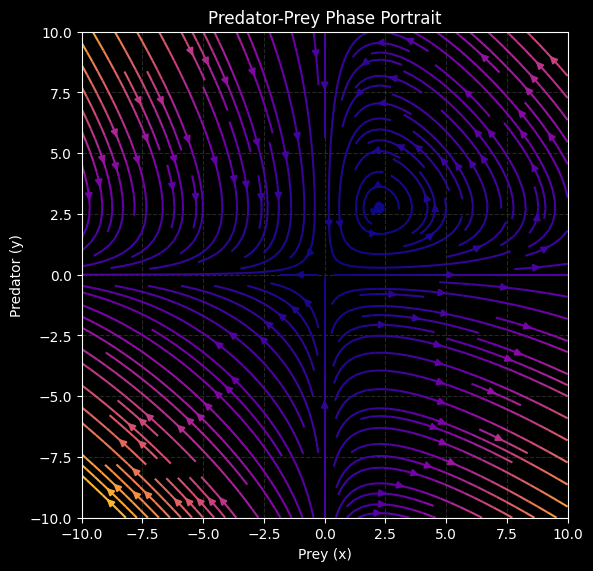
\includegraphics[width=0.8\linewidth]{figures/lv_true.png}
  \caption{The ground truth vector field of the Lotka-Volterra dynamical system, 
  showing its characteristic stable cycle.}
  \label{fig:lv_true_vs_mlp}
  \Description{A phase portrait plot showing the true spiral dynamics of the Lotka-Volterra system. 
  The vector field flows in a counter-clockwise spiral pattern.}
\end{figure}

\begin{figure}[h!]
  \centering
  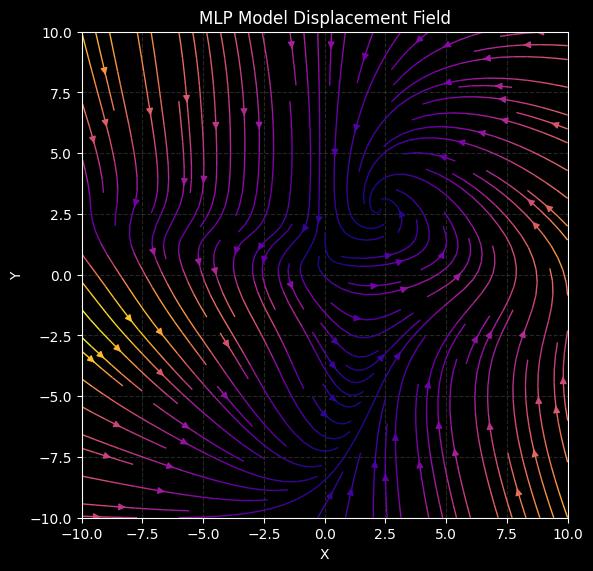
\includegraphics[width=0.8\linewidth]{figures/lv_mlp.png}
  \caption{The vector field learned by a standard MLP. 
  It fails to capture the rotational dynamics of the true system.}
  \label{fig:lv_mlp}
  \Description{A phase portrait plot from a standard MLP, 
  showing a distorted, non-rotational vector field.}
\end{figure}

Next, we evaluate two NODE-based models, differing only in their activation function. 
The results in Figures~\ref{fig:lv_tanh} and \ref{fig:lv_relu} are striking. 
The Tanh-based NODE captures a distorted sense of rotation but fails to accurately model the system. 
In contrast, the ReLU-based NODE almost perfectly reconstructs the vector field. 
This result confirms that NODEs possess a powerful inductive bias for learning continuous vector 
fields, but their success is highly dependent on both the problem domain and key architectural choices.

\begin{figure}[h!]
  \centering
  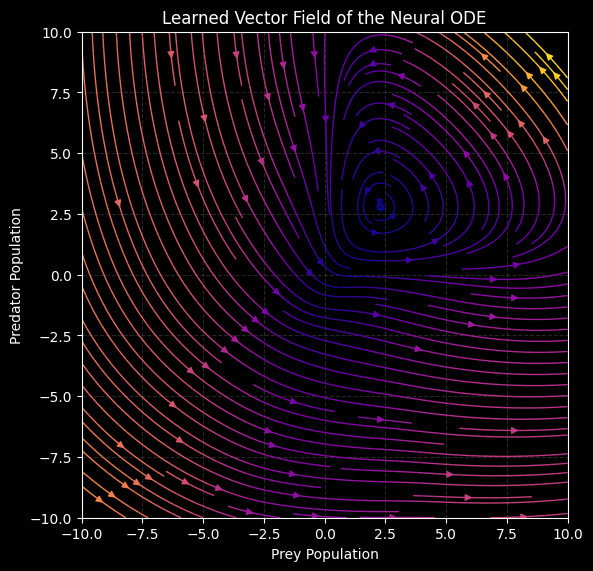
\includegraphics[width=0.8\linewidth]{figures/lv_tanh.png}
  \caption{The learned vector field from a NODE with a Tanh activation function. 
  The dynamics are distorted and inaccurate.}
  \label{fig:lv_tanh}
  \Description{A phase portrait plot from a Tanh-based NODE, showing a distorted spiral pattern.}
\end{figure}

\begin{figure}[h!]
  \centering
  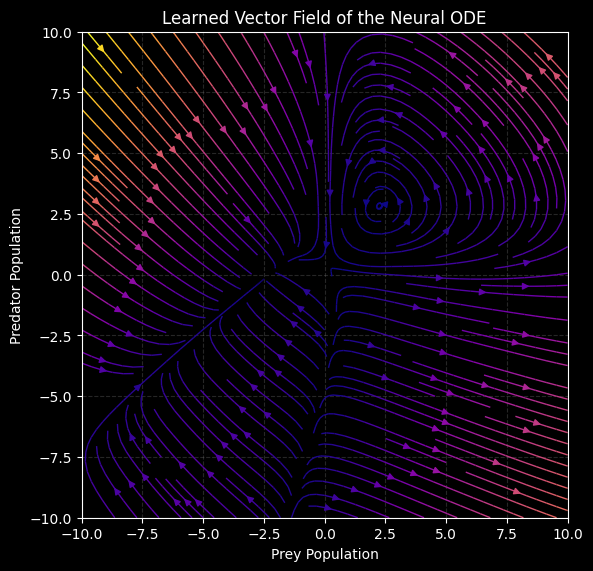
\includegraphics[width=0.8\linewidth]{figures/lv_relu.png}
  \caption{The learned vector field from a NODE with a ReLU activation function. 
  The model accurately reconstructs the true dynamics.}
  \label{fig:lv_relu}
  \Description{A phase portrait plot from a ReLU-based NODE, showing nearly perfect 
  spiral patterns identical to the ground truth.}
\end{figure}